\chapter{Oscil·lacions}
\section{Moviment Harmònic Simple.}
Ara no tinc temps per explicar merdes, però tens un potencial i té un mínim i volem saber com es mouen les coses al voltant d'aquest mínim. Expandim per Taylor i queden expressions com
\[
F(x)=-\dfrac{E_p}{dx}\approx-kx,\quad F=ma=m\dfrac{d^2x}{dt^2}=-kx
\]
i d'aquí l'\textit{equació del moviment harmònic simple},
\[
\ddot x+\dfrac{k}{m}x=0.
\]
Es prova una solució del tipus $x=Ae^{\lambda t}$, en surten dues, així que les superposem, i queda
\[
x=c_1e^{\lambda_1t}+c_2e^{\lambda_2t},\quad\lambda=\pm i\sqrt{\dfrac{k}{m}}.
\]
Diem $\omega_0=\sqrt{\dfrac{k}{m}}$. La solució general és per tant
\[
x(t)=Ae^{i\omega_0t}+Be^{-i\omega_0t}=A(\cis(\omega_0t))+B(\cis(-\omega_0t))=(A+B)\cos(\omega_0t)+i(A-B)\sin(\omega_0t)
\]\[=C\cos(\omega_0t)+D\sin(\omega_0t)=\boxed{A'\cos(\omega_0t+\delta).}\]
Direm $T=\dfrac{2\pi}{\omega_0}$ el \textit{període d'oscil·lació}.
\subsection{Energia del MHS.}
\[
E_p=\dfrac{1}{2}kx^2=\dfrac{1}{2}kA^2\cos^2(\omega_0t+\delta),\quad E_c=\dfrac{1}{2}mv^2=\dfrac{1}{2}mA^2\omega_0^2\sin^2(\omega_0t+\delta)\implies
\]
\[
E=E_p+E_c=\dfrac{1}{2}kA^2,\quad A=\sqrt{\dfrac{2E}{k}}.
\]
\section{Oscil·lacions harmòniques en dues dimensions.}
En dues dimensions tindrem
\[F=-k\vec r=-kr\hat r=-k(x\hat i+y\hat j),\]
i per tant les equacions
\[
\begin{cases}
m\ddot x+kx=0\implies x(t)=A\cos(\omega_0t+\delta),\\
m\ddot y+ky=0\implies y(t)=B\cos(\omega_0t+\gamma).
\end{cases}
\]
Si triem l'origen del temps tal que $\gamma = 0$,
\[
\begin{cases}
x(t)=A\cos(\omega_0t+\delta),\\
y(t)=B\cos(\omega_0t);
\end{cases}
\implies
x(t)=A[\cos(\omega_0t)\cos{\delta}-\sin(\omega_0t)\sin{\delta}]\]\[=A\left[\dfrac{y}{B}\cos{\delta}-\sqrt{1-\dfrac{y^2}{B^2}}\sin{\delta}\right]
\implies(\cdots)\implies\]
\[\boxed{x^2+\dfrac{A^2}{B^2}y^2-2\dfrac{A}{B}xy\cos{\delta}=A^2\sin^2{\delta}.}\]
\section{Oscil·lacions amortiguades.}
Suposem un amortiguament proporcional a la velocitat, $F=-bv$. L'equació del moviment queda
\[
m\ddot x=-kx-b\dot x\implies\ddot x+\dfrac{b}{m}\dot x+\dfrac{k}{m}x=0.
\]
Definirem $\omega_0^2=\dfrac{k}{m},\ \beta=\dfrac{b}{2m}$, i aleshores tenim
\[
\boxed{
\ddot x+2\beta\dot x+\omega_0^2x=0.
}
\]
Suposem una solució $x(t)=Ae^{\lambda t}$, i la solució general de l'equació de sobre és
\[
\lambda=-\beta\pm\sqrt{\beta^2-\omega_0^2},\quad x(t) = Ae^{\lambda^+t}+Be^{\lambda^-t}=e^{-\beta t}(Ae^{\sqrt{\beta^2-\omega_0^2}t}+Be^{-\sqrt{\beta^2-\omega_0^2}t}).
\]
Definim
\begin{itemize}
	\item \textbf{Oscil·lacions sobreamortiguades:} En les que $\beta^2>\omega_0^2$.
	\item \textbf{Oscil·lacions crítiques:} En les que $\beta^2=\omega_0^2$. Aquí, $x(t)=(A+Bt)e^{-\beta t}$.
	\item \textbf{Oscil·lacions subamortiguades:} En les que $\beta^2<\omega_0^2$.
\end{itemize}
En aquestes últimes, si $\omega = \sqrt{\omega_0^2-\beta^2}$,
\[
x(t)=e^{-\beta t}(Ae^{\sqrt{\beta^2-\omega_0^2}t}+Be^{-\sqrt{\beta^2-\omega_0^2}t})=e^{-\beta t}(C\cos(\omega t)+D\sin(\omega t))=e^{-\beta t}A'\cos(\omega t+\delta)=A'(t)\cos(\omega t+\delta).
\]
Si $\beta << \omega$, $v(t)\approx-A\omega e^{-\beta t}\sin(\omega t+\delta)$. L'energia és $E=\dfrac{1}{2}kA^2e^{-2\beta t}$.
\section{Oscil·lacions forçades.}
Suposarem un oscil·lador harmònic subamortiguat subjecte a un forçat extern periòdic. Suposarem que tenim una força sinusoidal, $F=F_0\cos(\omega_F t)$. L'equació del moviment serà
\[\boxed{\ddot x+2\beta\dot x+\omega_0^2x=A\cos(\omega_F t),}\quad A = \dfrac{F_0}{m}.\]
La solució general serà
\[\boxed{
	x(t)=x_h(t)+x_p(t),
}\]
respectivament solució de l'equació homogènia i solució particular. Suposarem
\[\begin{cases}x_p(t)=D\cos(\omega_Ft-\delta),\\ \dot x_p=-\omega_FD\sin(\omega_Ft-\delta),\\ \ddot x_p=-\omega_F^2D\cos(\omega_Ft-\delta).\end{cases}\]
Per a ser solució ha de complir l'equació
\[\text{insertar substitució en l'equació}\]
\[(\cdots)\iff D=\dfrac{A}{\sqrt{(\omega_0^2-\omega_F^2)^2+4\omega_F^2\beta^2}},\quad \tan{\delta}=\dfrac{2\beta\omega_F}{\omega_0^2-\omega_F^2}.\]
\textbf{Freqüència de ressonància:} aquella que maximitza $D$. És [insertar càlculs]
\[
\omega_R=\sqrt{\omega_0^2-2\beta^2},
\]
i $D$ val
\[D_{\text{max}}=\dfrac{F_0}{2m\beta\sqrt{\omega_0^2-\beta^2}}.\]
\subsection{Superposició de forces.}
Les oscil·lacions forçades satisfan una equació de la forma
\[
\boxed{
	\left(\dfrac{d^2}{dt^2}+2\beta\dfrac{d}{dt}+\omega_0^2\right)x(t)=A\cos(\omega_Ft).
}
\]
A l'operador entre parèntesi l'anomenarem $\mathcal L$. Per tant, tenim que l'equació satisfeta per les oscil·lacions forçades és
\[
\mathcal L x(t)=F(t).
\]
$\mathcal L$ és lineal (superposició, producte per constant, etc). Si la força externa es pot representar com la suma de diverses forces,
\[
F(t)=\sum_{i=1}^m\alpha_iF_i(t)\implies x(t)=\sum_{i=1}^m\alpha_ix_i(t),
\]
sent sempre que $\mathcal L x_i(t)=F_i(t)$. Donada una força periòdica, podem escriure-la en sèrie de Fourier com
\[
F(t)=\dfrac{1}{2}a_0+\sum_{n\geq1}(a_n\cos(n\omega t)+b_n\sin(n\omega t)),
\]
sent
\[
a_n=\dfrac{2}{T}\int_0^TF(s)\cos(n\omega s)ds,\quad
b_n=\dfrac{2}{T}\int_0^TF(s)\sin(n\omega s)ds.
\]
\section{Oscil·lacions acoplades}
Acoplament de dos oscil·ladors harmònics:
\begin{center}
  \makebox[\textwidth]{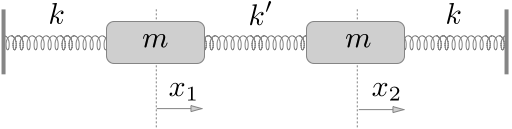
\includegraphics[width=0.5\textwidth]{coupled-oscillators.png}}
\end{center}
\[
F_1=-kx_1+k'(x_2-x_1),\quad F_2=-kx_2-k'(x_2-x_1).
\]
Les equacions del moviment són
\[
\begin{cases}
m\ddot x_1+(k+k')x_1-k'x_2=0,\\
m\ddot x_2+(k+k')x_2-k'x_1=0.\\
\end{cases}
\]
Les solucions generals,
\[
x_1=B_1e^{\lambda t},\quad x_2=B_2e^{\lambda t},
\]
i suposarem $\lambda=i\omega$. Substituint a les equacions, passen coses, estan a la llibreta. El fet és que $B_1$ i $B_2$ són diferents de zero sii
\[
\omega^2=\dfrac{k}{m}\text{ o,}\quad\omega^2=\dfrac{k+2k'}{m},
\]
les anomenades \textit{freqüències normals}.
\begin{itemize}
	\item Si $\omega^2=\dfrac{k}{m}$, aleshores $\boxed{B_1=B_2}$ i $\boxed{x_1=x_2}$. (\textit{Oscil·lacions en fase})
	\item Si, pel contrari, $\omega^2=\dfrac{k+2k'}{m}$, aleshores $\boxed{B_1=-B_2}$ i $\boxed{x_1=-x_2}$. (\textit{Oscil·lacions en oposició de fase})
\end{itemize}
La solució general serà
\[
\begin{pmatrix}x_1\\ x_2\end{pmatrix}=\begin{pmatrix}1\\ 1\end{pmatrix}B_1\cos(\omega_1t+\delta)+\begin{pmatrix}1\\ -1\end{pmatrix}B_2\cos(\omega_2t+\delta).
\]
Fent un canvi de coordenades, $\eta_1=x_1-x_2,\ \eta_2=x_1+x_2$ (els \textit{modes normals}), passen coses i
\[
\begin{pmatrix}\eta_1\\ \eta_2\end{pmatrix}=\begin{pmatrix}2B_2\cos(\omega_2t+\delta)\\ 2B_1\cos(\omega_1t+\delta)\end{pmatrix},\quad\begin{pmatrix}\omega_1\\ \omega_2\end{pmatrix}=\begin{pmatrix}\sqrt{\dfrac{k}{m}}\\ \sqrt{\dfrac{k+2k'}{m}}\end{pmatrix}.
\]
\section{Ones.}
Passen coses. Amb una corda discreta. Llibreta. Algun dia les apuntaré. La qüestió és que l'\textcolor{red}{\textit{equació d'ones}} és
\[
\boxed{
	\dfrac{\partial^2q}{\partial t^2}=\dfrac{T}{\rho}\dfrac{\partial^2q}{\partial x^2}=v^2\dfrac{\partial^2q}{\partial x^2}.
}
\]
\textcolor{red}{Solucions de l'equació d'ones:} qualsevol funció de la forma $q(x-vt)$ o $q(x+vt)$.
\subsection{Ones harmòniques.}
\[
f(x,t)=A\sin(kx-\omega t)=A\sin(k(x-vt)),\quad v=\dfrac{\omega}{k},T=\dfrac{2\pi}{\omega}=\dfrac{2\pi}{vk},\lambda=\dfrac{2\pi}{k}.
\]
\subsection{Equacions de Maxwell en absència de càrregues i corrents.}
\textit{"Otro día, vale?"}